\section{Problem formulation}\label{sec:continuous}
As an illustrative example of our technique, we consider the scenario illustrated in \cref{fig:domain}. 
\begin{figure}%
  \centering
  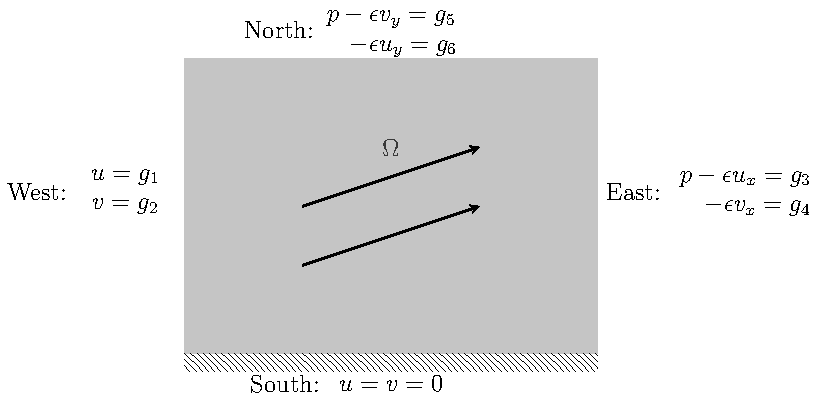
\includegraphics[width=0.7\textwidth]{images/domain/domain.pdf}
  \caption{Illustration of the computational domain $\Omega$ and the specific boundary conditions.}%
  \label{fig:domain}
\end{figure}
An incompressible fluid is moving from left to right. Hence, the left side is an inflow boundary, where Dirichlet conditions are imposed, and the right side is an outflow boundary, where natural boundary conditions \cite{papanastasiou1992new} are imposed. The lower part of the domain is a no-slip wall and the upper side is an outflow boundary, where again natural conditions are imposed. The initial-boundary value problem for the INS equations that we consider is
\begin{equation}
\begin{aligned}
  \tilde{I} \w_t  + \eul(\w)	& = 0
	& \quad & (x,y) \in \Omega, & \quad t & > 0
	\\
	\mathcal{H} \w & =  \g & \quad & (x,y) \in \partial\Omega, & \quad t & > 0
	\\
  \tilde{I} \w 	& =  \tilde{I}\f & \quad & (x,y) \in \Omega, & \quad t & = 0
	\, .
\end{aligned} 
\label{eq:ins_continuous}
\end{equation}
In \eqref{eq:ins_continuous}, $\w = (u,v,p)^\top$, where $u,v$ are the velocities in the $x,y$ direction, respectively, and $p$ is the pressure. Furthermore, $\Omega = [0,1]^2$ is the domain and $\partial \Omega$ its boundary. The initial data $\f$ and boundary data $\g$ are sufficiently smooth and compatible functions and the spatial operator is given by \cite{nordstrom2019energy}
\begin{equation}
  \eul(\w) = 
  \frac{1}{2}\left[A \w_x + (A \w)_x + B \w_y + (B \w)_y\right] 
  - \epsilon\tilde{I}[\w_{xx} + \w_{yy}]
  \, .
  \label{eq:eul}
\end{equation}
The matrices in \eqref{eq:ins_continuous} and $\eqref{eq:eul}$ are 
\[
   A = 
   \begin{pmatrix}
      u & 0 & 1
      \\
      0 & u & 0
      \\
      1 & 0 & 0
   \end{pmatrix}
   , \quad 
   B = 
   \begin{pmatrix}
      v & 0 & 0
      \\
      0 & v & 1
      \\
      0 & 1 & 0
   \end{pmatrix}
   ,\quad 
   \tilde{I} = 
   \begin{pmatrix}
      1 & 0 & 0
      \\
      0 & 1 & 0
      \\
      0 & 0 & 0
   \end{pmatrix}
   \, .
\]
Lastly, the explicit form of the boundary conditions $\mathcal{H}\w = \g$ reads
\begin{equation}
\begin{aligned}
  u & = g_1 \quad & v & = g_2  & \quad & \text{at}  \quad x = 0 \quad && \text{(West)}
  \\
  p - \epsilon u_x & = g_3 \quad & -\epsilon v_x & = g_4 & \quad & \text{at} \quad x = 1  \quad && \text{(East)}
  \\
  u &= 0 \quad & v &= 0        & \quad & \text{at}  \quad y = 0 \quad && \text{(South)}
  \\
  p-\epsilon v_y &= g_5 \quad & -\epsilon u_y &= g_6        & \quad & \text{at}  \quad y = 1 \quad && \text{(North)}
  \, .
\label{eq:boundary_conditions}
\end{aligned}
\end{equation}

\subsection{Boundedness}
We will for completeness show how to bound the solution. For simplicity, only the south side of the domain is discussed explicitly. Details of the upcoming analysis are found in \cite{nordstrom2019energy}. 

For two vector functions $\phiv,\psiv$ defined on $\Omega$, we introduce the inner product and norm
\[
  \langle \phiv, \psiv \rangle = \int_\Omega \phiv^\top \psiv d\Omega
  , \quad
  \|\phiv\|^2 = \langle \phiv,\phiv\rangle
  \, .
\]
By multiplying \eqref{eq:ins_continuous} by $2\w^\top$ from the left and integrating over $\Omega$, we get
\begin{equation}
   \frac{d}{dt}\|\w\|^2_{\It} + 2\epsilon \|\nabla \w\|^2_{\It} =  BT
   \, ,
   \label{eq:energy_continuous}
\end{equation}
where $\nabla \w = (\nabla u,\nabla v, \nabla p)^\top$, $\|\nabla \w\|^2_{\It}$ is a dissipative volume term and
\[
  BT = 
  \int_{\text{South}}\w^\top (B \w - 2\epsilon \It \w_y) d x
\]
contains the boundary terms evaluated at the south boundary. The other boundary terms are assumed dissipative and ignored. Imposing $u = v = 0$ results in $BT = 0$. Integrating \eqref{eq:energy_continuous} in time (assuming homogeneous boundary conditions on all sides) leads to 
\begin{equation}
   \|\w\|^2_{\tilde{I}}(T) + 2\epsilon \int_0^T\|\nabla \w\|^2_{\tilde{I}} dt
   \le  \|f\|_{\tilde{I}}^2
   \, ,
   \label{eq:estimate_continuous}
\end{equation}
which bounds the semi-norm of the solution ($\|\w\|^2_{\tilde{I}}$) and its gradients ($\|\nabla \w\|^2_{\tilde{I}}$) for any time.
